\documentclass{article}
\usepackage[T1]{fontenc}
\usepackage[utf8x]{inputenc}
\usepackage{amsmath}
\usepackage{amsthm}
\theoremstyle{plain}
\usepackage{enumitem}
\usepackage[OT4]{polski}
\usepackage{caption}
\usepackage{subcaption}
\usepackage{tabularx}
\usepackage{caption}
%\captionsetup[table]{skip=-4pt}
\usepackage{tabulary}
\usepackage{array}
\usepackage{hyperref}
\usepackage[pdftex]{graphicx}
\usepackage{sidecap}

\usepackage{wrapfig}

\newtheorem{ciekaw}{Ciekawostka}

\newcolumntype{L}[1]{>{\raggedright\let\newline\\\arraybackslash\hspace{0pt}}m{#1}}
\newcolumntype{C}[1]{>{\centering\let\newline\\\arraybackslash\hspace{0pt}}m{#1}}
\newcolumntype{R}[1]{>{\raggedleft\let\newline\\\arraybackslash\hspace{0pt}}m{#1}}

\usepackage[justification=centering]{caption}
\usepackage{graphicx}
\usepackage{lastpage}
\usepackage{fancyhdr}
\usepackage{gensymb}

%\pagestyle{fancy}

\usepackage[margin=60pt]{geometry}

\begin{document}
\section{Co to jest klimat?}
Klimatem nazywamy średnie warunki pogodowe obserwowane w danym miejscu na przestrzeni lat. \\
Przykładowe czynniki: temperatura, opady, zachmurzenie, wilgotność.
Modele klimatu są uproszonym opisem skomplikowanych procesów.
Klimat dzielimy na pięć części:
\begin{itemize}
	\item \textbf{Atmosfera} Gazowa część ponad powierzchnią ziemi.
	\item \textbf{Hydrosfera} Wszystkie formy wody nad i pod powierzchnią ziemi. 
	\item \textbf{Kriosfera} Wszystkie formy wody w postaci lodu.
	\item \textbf{Powierzchnia lądowa}
	\item \textbf{Biosfera} Organizmy żyjące w hydrosferze oraz na powierzchni lądowej.
\end{itemize}
\begin{figure}[h]
\begin{center}
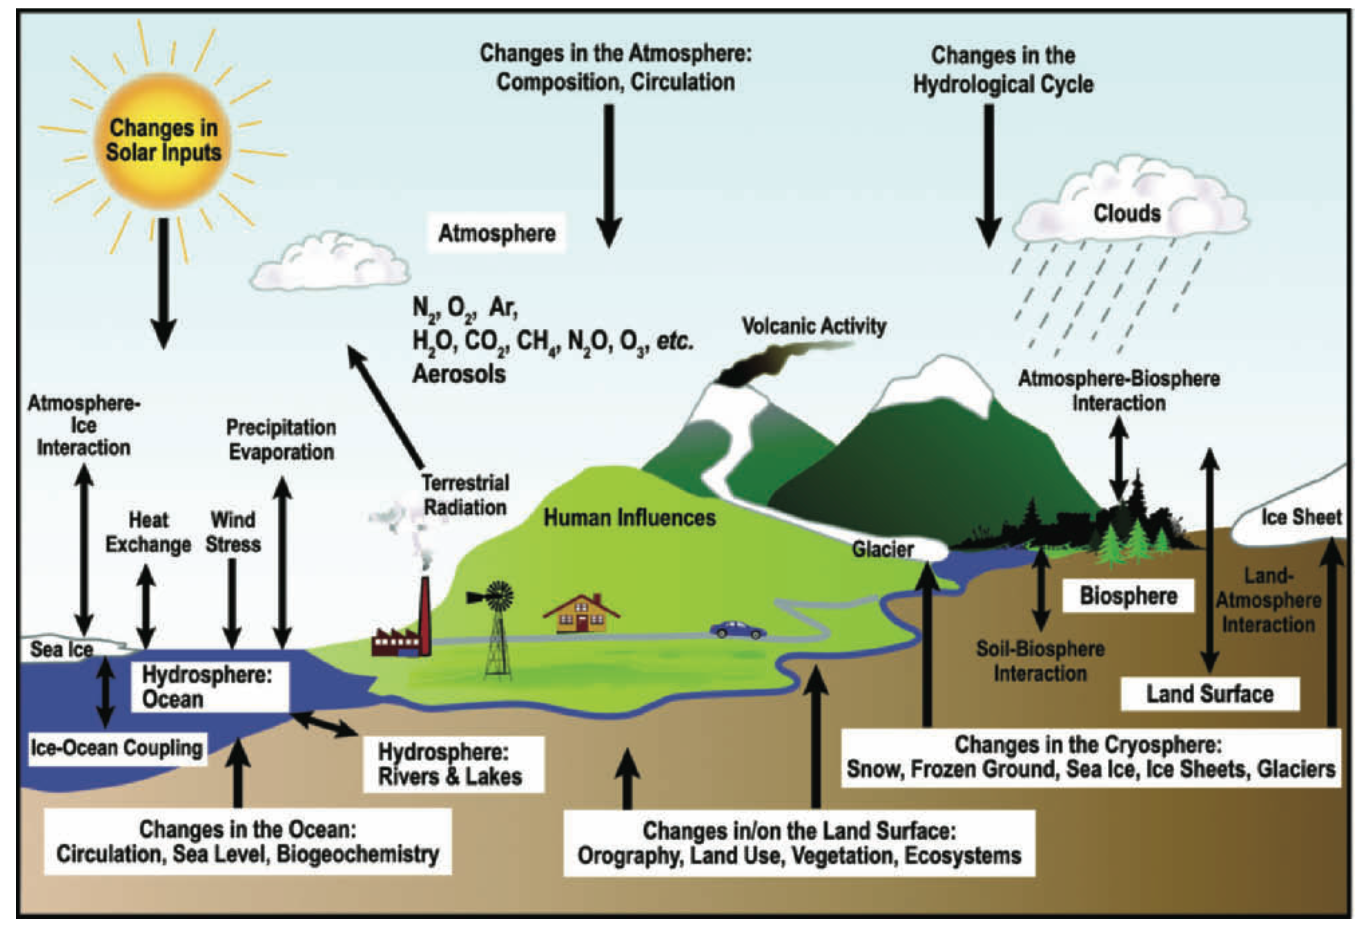
\includegraphics[width=0.7\linewidth]{images/Figure1}
\caption{Czynniki definiujące i wpływające na klimat}
\end{center}

\end{figure}

Na klimat najbardziej wpływają czynniki:
\begin{itemize}
	\item \textbf{Zmiany w promieniowaniu słonecznym} - "Changes in Solar inputs"
	\item \textbf{Promieniowanie ziemskie} - naturalne promieniowanie ziemskie
	\item \textbf{Zmiany w składzie gazowym atmosfery} - $N_2$,$O_2$,$CO_2$ itp. + aerozole.
\end{itemize}
Powyższe występują głównie w atmosferze. Ich zmiany prowadzą do zmiany klimatu. Nierównomiernie padające promieniowanie słoneczne oraz rotacja i pofałdowana powierzchnia lądów i oceanów  powoduje poziomy transport energii przez wodę i powietrze. Obecnie obserwowana zmiana klimatu jest połączeniem naturalnej wariacji oraz wpływu człowieka.
\begin{ciekaw}
	Naturalne zmiany klimatu można obserwować poprzez analizę okresu sprzed rewolucji przemysłowej (1750). - brak wpływu człowieka.
\end{ciekaw}
\begin{ciekaw}
IPPC - \textbf{Intergovernmental Panel on Climate Change} - organizacja założona w 1988 przez dwie organizacje Narodów Zjednoczonych – Światową Organizację Meteorologiczną (WMO) oraz Program Środowiskowy Organizacji Narodów Zjednoczonych (UNEP) w celu oceny ryzyka związanego z wpływem człowieka na zmianę klimatu.	
\end{ciekaw}
\subsection{Model klimatu}
Ogólnie model klimatu jest zdefiniowany jako matematyczna reprezentacja klimatu oparta na fizycznych, biologicznych i chemicznych zasadach. Dane dostarczone są tak złożone, że muszą być rozwiązane numerycznie. Konsekwencją tego faktu jest dyskretyzacja przestrzeni i czasu. (Modele odnoszą się do danego regionu, którego rozmiar zależy od rozdzielczości).
	\begin{figure}[h]
		\begin{center}
			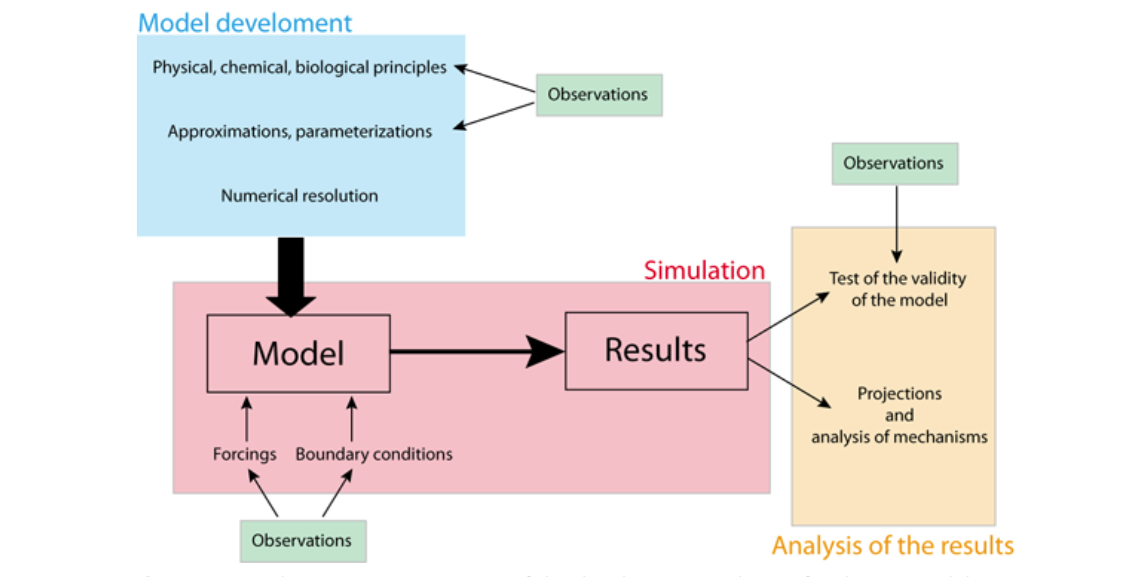
\includegraphics[width=1.0\linewidth]{images/Figure9}
			\caption{Proces tworzenia i weryfikowania modelu klimatu}
		\end{center}
	\end{figure}


\section{Pionowa struktura atmosfery}
Rozciąga się na całym obwodzie Ziemie (40000 km) i 100 km w górę.
\begin{figure}[h]
\begin{center}
	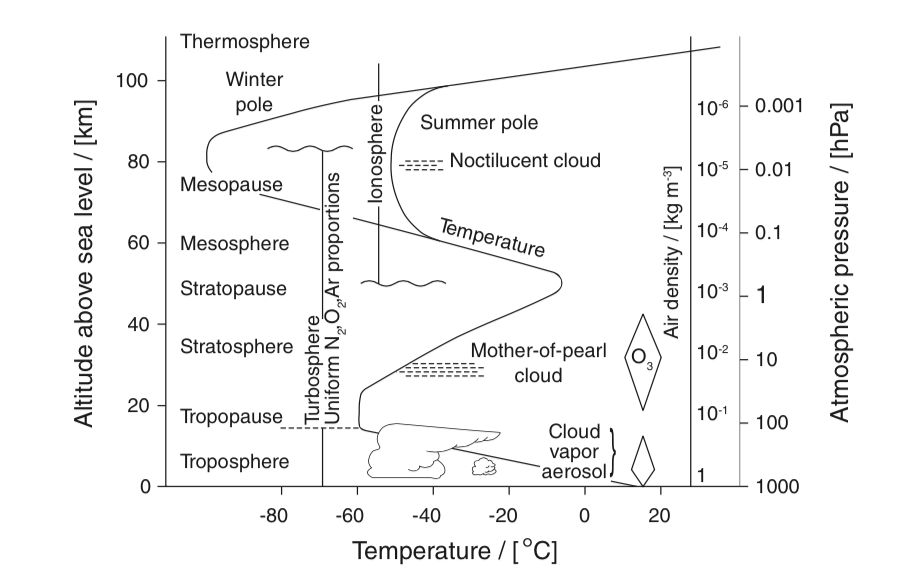
\includegraphics[width=0.7\linewidth]{images/Figure2}
	\caption{Pionowa struktura atmosfery}
\end{center}
\end{figure}
\begin{ciekaw}
	Temperatura powyżej 80km rośnie, ponieważ $O_2$ fotodysocjuje w $O$, które silnie pochłania promieniowania o $\lambda \in(100,200)$ nm.	
\end{ciekaw}

\section{Modelowanie Atmosfery}
AGCMs - \textit{(atmospheric) General Circulation Model} - \textbf{Model ogólnej cyrkulacji}
	Rozwiązanie tych równań daje:
	\begin{itemize}
		\item ciśnienie atmosferyczne
		\item prędkość i kierunek wiatru
		\item temperaturę i wilgotność na różnych poziomach
	\end{itemize}
	Atmosferę opisuje siedem zmiennych opisanych za pomocą siedmiu równań. ($\overrightarrow{v} = (u,v,w)$, ciśnienie - $p$, temperatura $T$, wilgotność $q$, gęstość - $\rho$).\\
	Zachowanie pędu ( z II zasady dynamiki Newtona):
	\begin{equation}
		\frac{D\overrightarrow{v}}{Dt} = -\frac{1}{\rho}\overrightarrow\nabla p - \overrightarrow{g} + \overrightarrow{F_{tarcia}} - 2\overrightarrow{\Omega}\times\overrightarrow{v}
	\end{equation}
	$\Omega$ - prędkość kątowa wektora Ziemi - siła Coriolisa. $F$ - siła tarcia\\
	Zasada zachowania masa:
	\begin{equation}
		\frac{\partial p}{\partial t} = -\overrightarrow{\nabla}(\overrightarrow{\rho v})
	\end{equation}


\subsection{Skończona siatka}
	Nie można dokładnie (analitycznie) rozwiązać równań ruchu powietrza w ogólnym przypadku. Numeryczne (komputerowe) rozwiązania wymagają dyskretyzacji za pomocą różnych przybliżeń numerycznych, np różnic skończonych, metod spektralnych lub elementów skończonych. Typowa rozdzielczość AGCM to 1-5 stopnia szerokości i długości geograficznej, czyli co około 100-500 km.
	Symulowanie za pomocą pudeł jest jedną z najprostszych metod. Atmosfera zostaje zredukowana do pewnych zbiorów zmiennych równo rozmieszczonych w danych pudłach. Każda kolumna jest podzielona na rzędy(layers). Kolejne rzędy mają kształt terenu, na którym stoi kolumna(współrzędne sigma)
\begin{figure}[h!]
\begin{center}
	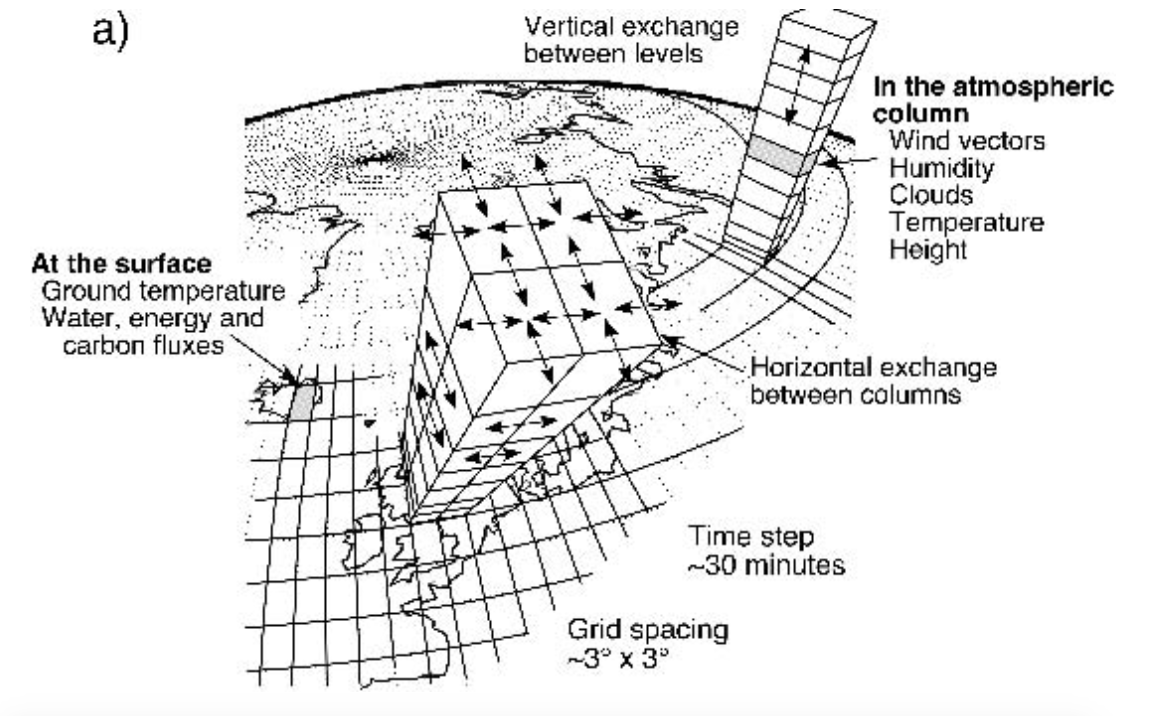
\includegraphics[width=0.7\linewidth]{images/Figure3}
	\caption{Konstrukcja siatki AGCM}
\end{center}
\end{figure}
\begin{figure}[h!]
\begin{center}
	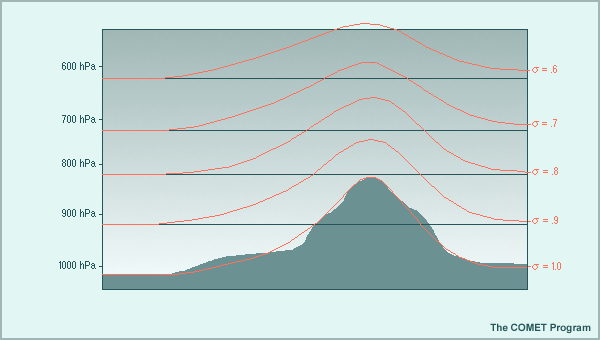
\includegraphics[width=0.7\linewidth]{images/Figure4}
	\caption{Współrzędne sigma}
\end{center}
\end{figure}
\begin{ciekaw}
	Ostatnio w modelowaniu zamiast sześcianów zaczęto używać 20-stościanów.
\end{ciekaw}
Odstępy czasu w takim modelowaniu muszą być wystarczająco krótkie, tak aby z jednego do drugiego pudła nie przechodziły informacje:
\begin{equation}
	\Delta t \le \Delta x/c
\end{equation}
Gdzie $\Delta x$ jest szerokością pudła. 
Taki model jest używany zazwyczaj w OGCM, ale pierwszy model atmosfery był wykonany w ten sposób. Powszechnie używa się modeli spektralnych.
\subsection{Modele spektralne}
	Znajdują zastosowanie w modelowaniu atmosfery, ponieważ przyjmuje ona kształt okrągłej powłoki powietrza, co sugeruje użycie współrzędnych sferycznych.
	Atmosfera jest podzielona na kawałki manipulowane jako fale. Co przyśpiesza i ułatwia obliczenia. Taki sposób jest wykorzystywany tylko przy wymianie poziomej. Przy pionowej nadal wygodnie jest używać siatki.  

\subsection{Opis równań}
\begin{itemize}
	\item \textbf{Równanie gazu dosknałego}
	\item \textbf{Zasada zachowania masy}\\
		Materia nie może zostać 
\end{itemize}


\section{Modelowanie oceanu}
	Ocean jest 'sterowany' przez:
	\begin{itemize}
		\item Siła mechaniczna wiatru
		\item Wypadkowy efekt gęstości i zasolenia wody
		\item Wymiana ciepła z atmosferą
		\item Wilgotność
	\end{itemize}
Prąd(pływ oceanu) jest wynikiem powyższych oraz ruchu obrotowego Ziemi.(Silny na zachodnie stronie basenów oceanu). Temperatura, zasolenie mają swoje maksima właśnie w centrum tych prądów. 
Modele oceanu: dwuwymiarowe, trójwymiarowe.

\section{Modelowanie Kriosfery}
Najbardziej dynamicznym elementem są polarne lodowce. Taki model musi uwzględniać, pokrywę śnieżną, lodowce i lądolody. Słaba dokładność: procesy trwają kilkaset lat.
Własności kriosfery:
\begin{itemize}
	\item Śnieg i lód mają wysokie albedo - są istotne w globalnym balansie ciepła. 
	\item Zwiększają wymianę ciepła i gazów pomiędzy oceanami a atmosferą.
\end{itemize}

	\begin{figure}[h]
		\begin{center}
			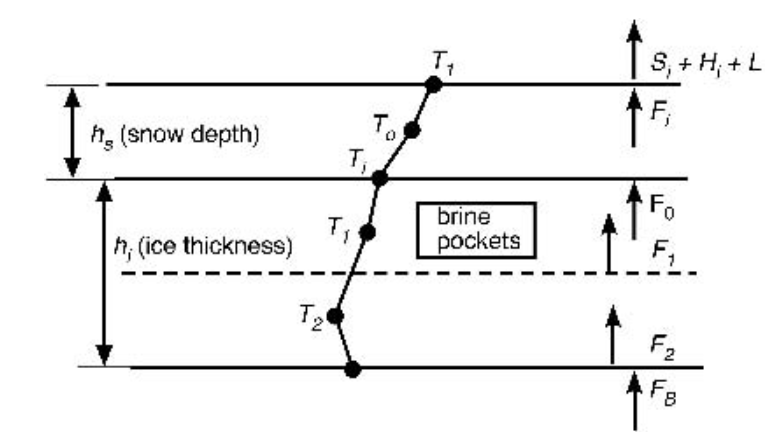
\includegraphics[width=0.8\linewidth]{images/Figure7.png}
			\caption{Najprostszy model to trójwarstowy model termodynamiczny}
		\end{center}
	\end{figure}
Przewiduje dwie temperatury lodu, temperaturę śniegu, natomiast temperatura oceanu pozostaje stała.


\subsection{Modelowanie powierzchni lądowej}
























\end{document}